% !TeX spellcheck = en_GB
\begin{figure}[t]
	\centering
    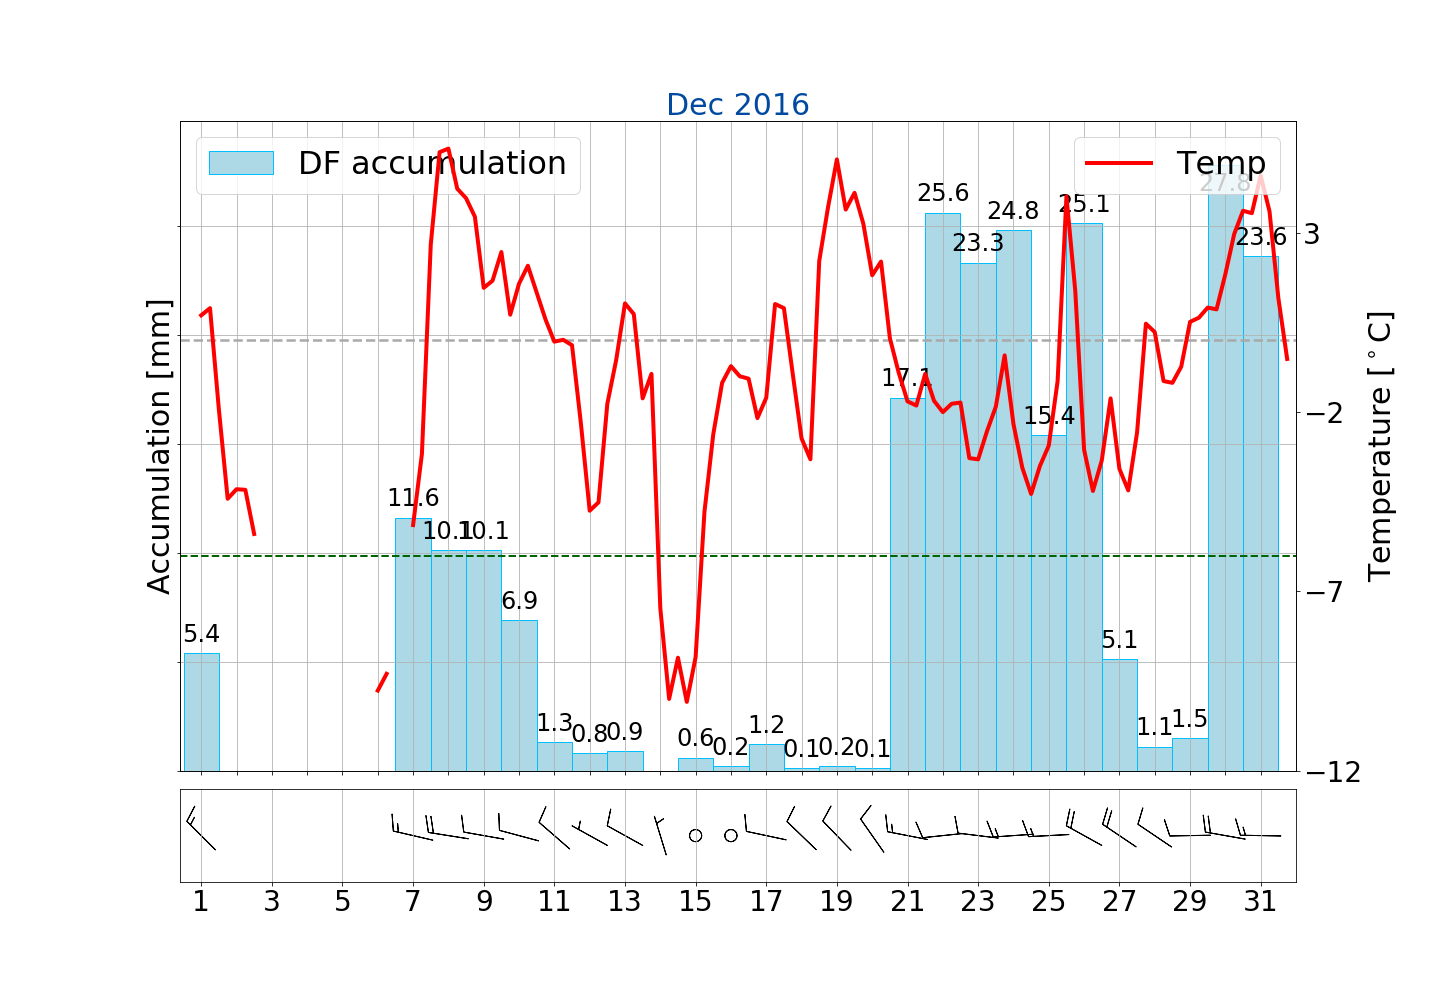
\includegraphics[trim={4.cm 3.3cm 1.5cm 3.cm},clip,
        width=0.8\textwidth]{./fig_weathermast/T_P_U_201612}
        \caption{Observations at Haukeliseter weather mast for December 2016. Daily accumulation [\SI{}{\mm}] in light blue, mean temperature every six hours (red, [\SI{}{\celsius}]), and daily maximum wind as barbs [\SI{}{\mPs}]. Gray dashed line indicates the freezing temperature. The monthly normal value is green dashed (\SI{-6.0}{\celsius}), the values are taken from \cite{eklima_norwegian_2016}. Note, that no data was available from \SIlist{2;6}{\dec}} \label{fig:DecObs}
\end{figure}